% binary_clock.tex
% My first AVR project. This is the whole document.

\documentclass[11pt,a4paper]{article}

\usepackage{graphicx}
\usepackage{indentfirst}
\usepackage{verbatim}
%\usepackage{multirow}
%\usepackage{fancybox}
%\usepackage{endnotes}

\title{Binary Clock: RTC of ATmega48 and LED DISPLAY}
\author{sun\_ge@yahoo.cn}

\begin{document}

\maketitle

\begin{center}
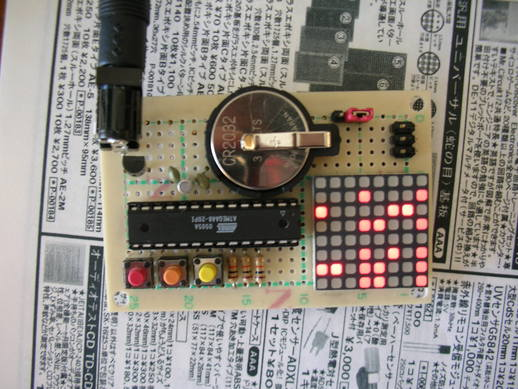
\includegraphics{binclock.jpg}
\end{center}

\section{Project Origin}
A few years ago, I found some kinds of binary clock for sale in ~\textit{www.thinkgeek.com}~,
then I tried to write a J2ME clock software that can show time by flashing green dot in my cell phone.
When I knew the advantage of microcontroller just as ATmega48, I think it is very easy to 
make a hardware binary clock because: \\
\begin{enumerate}
\item ATmega48 has a asynchronous T/C2 which can use a 32768Hz watch crystal as independent clock source.
\item It has sufficient GPIO to drive a 8x8 LED dot-matrix display and three push button.
\item ATMEL provide a application note ~\textit{AVR134: Real-Time Clock using the Asynchronous Timer}~ and
example code.
\item It has another project "LCD Big-Number Clock" in the Internet, Its code can be useful.
\end{enumerate}

\section{Schematics}
You can enlarge it but I should confess that it's truely very ugly.

Instead of the schematics, source code also contain connection informations
and technical notes, please see it for details.\\

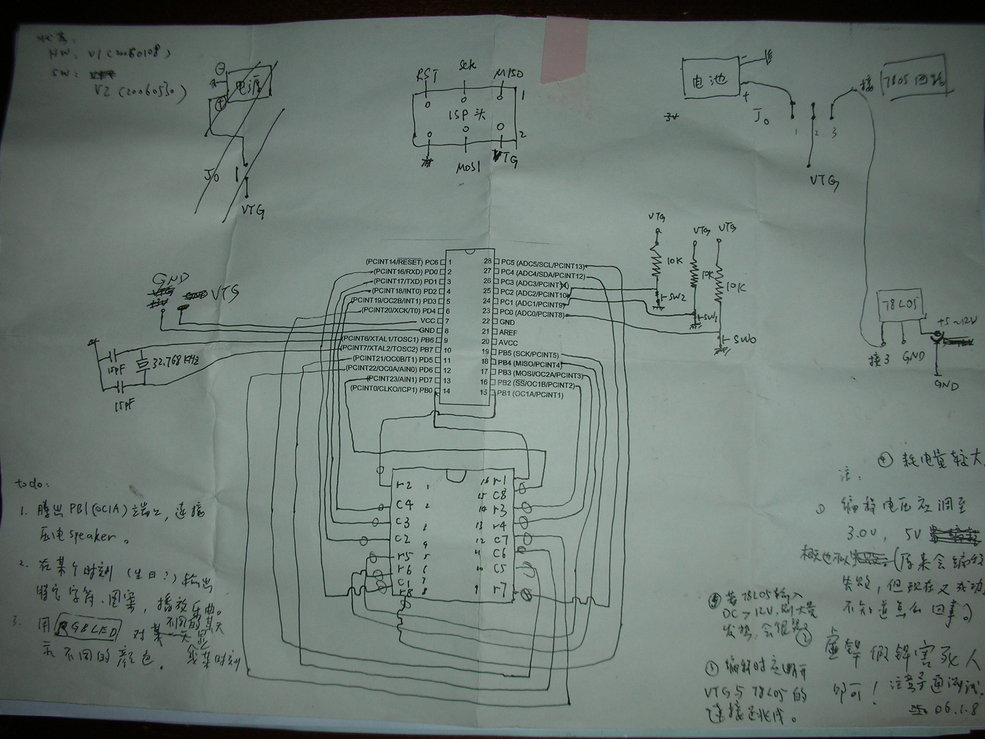
\includegraphics[scale=0.5]{binclock_sch.jpg}

\section{Source Code}
Source contains: rtcasync.c, rtcasync.h, binclock.c and Makefile.\\
It can be compiled and installed by AVR GNU Tools Chain.
\subsection{RTC Library: rtcasync.c}
\verbatiminput{rtcasync.c}

\subsection{RTC Library Header: rtcasync.h}
\verbatiminput{rtcasync.h}

\subsection{Main Program: binclock.c}
\verbatiminput{binclock.c}

\subsection{Makefile}
\verbatiminput{Makefile}

\end{document}

%%% Local Variables:
%%% coding: UTF-8
%%% mode: latex
%%% End:
